% Options for packages loaded elsewhere
\PassOptionsToPackage{unicode}{hyperref}
\PassOptionsToPackage{hyphens}{url}
\PassOptionsToPackage{dvipsnames,svgnames,x11names}{xcolor}
%
\documentclass[
  letterpaper,
  DIV=11,
  numbers=noendperiod]{scrreprt}

\usepackage{amsmath,amssymb}
\usepackage{iftex}
\ifPDFTeX
  \usepackage[T1]{fontenc}
  \usepackage[utf8]{inputenc}
  \usepackage{textcomp} % provide euro and other symbols
\else % if luatex or xetex
  \usepackage{unicode-math}
  \defaultfontfeatures{Scale=MatchLowercase}
  \defaultfontfeatures[\rmfamily]{Ligatures=TeX,Scale=1}
\fi
\usepackage{lmodern}
\ifPDFTeX\else  
    % xetex/luatex font selection
\fi
% Use upquote if available, for straight quotes in verbatim environments
\IfFileExists{upquote.sty}{\usepackage{upquote}}{}
\IfFileExists{microtype.sty}{% use microtype if available
  \usepackage[]{microtype}
  \UseMicrotypeSet[protrusion]{basicmath} % disable protrusion for tt fonts
}{}
\makeatletter
\@ifundefined{KOMAClassName}{% if non-KOMA class
  \IfFileExists{parskip.sty}{%
    \usepackage{parskip}
  }{% else
    \setlength{\parindent}{0pt}
    \setlength{\parskip}{6pt plus 2pt minus 1pt}}
}{% if KOMA class
  \KOMAoptions{parskip=half}}
\makeatother
\usepackage{xcolor}
\setlength{\emergencystretch}{3em} % prevent overfull lines
\setcounter{secnumdepth}{5}
% Make \paragraph and \subparagraph free-standing
\makeatletter
\ifx\paragraph\undefined\else
  \let\oldparagraph\paragraph
  \renewcommand{\paragraph}{
    \@ifstar
      \xxxParagraphStar
      \xxxParagraphNoStar
  }
  \newcommand{\xxxParagraphStar}[1]{\oldparagraph*{#1}\mbox{}}
  \newcommand{\xxxParagraphNoStar}[1]{\oldparagraph{#1}\mbox{}}
\fi
\ifx\subparagraph\undefined\else
  \let\oldsubparagraph\subparagraph
  \renewcommand{\subparagraph}{
    \@ifstar
      \xxxSubParagraphStar
      \xxxSubParagraphNoStar
  }
  \newcommand{\xxxSubParagraphStar}[1]{\oldsubparagraph*{#1}\mbox{}}
  \newcommand{\xxxSubParagraphNoStar}[1]{\oldsubparagraph{#1}\mbox{}}
\fi
\makeatother


\providecommand{\tightlist}{%
  \setlength{\itemsep}{0pt}\setlength{\parskip}{0pt}}\usepackage{longtable,booktabs,array}
\usepackage{calc} % for calculating minipage widths
% Correct order of tables after \paragraph or \subparagraph
\usepackage{etoolbox}
\makeatletter
\patchcmd\longtable{\par}{\if@noskipsec\mbox{}\fi\par}{}{}
\makeatother
% Allow footnotes in longtable head/foot
\IfFileExists{footnotehyper.sty}{\usepackage{footnotehyper}}{\usepackage{footnote}}
\makesavenoteenv{longtable}
\usepackage{graphicx}
\makeatletter
\newsavebox\pandoc@box
\newcommand*\pandocbounded[1]{% scales image to fit in text height/width
  \sbox\pandoc@box{#1}%
  \Gscale@div\@tempa{\textheight}{\dimexpr\ht\pandoc@box+\dp\pandoc@box\relax}%
  \Gscale@div\@tempb{\linewidth}{\wd\pandoc@box}%
  \ifdim\@tempb\p@<\@tempa\p@\let\@tempa\@tempb\fi% select the smaller of both
  \ifdim\@tempa\p@<\p@\scalebox{\@tempa}{\usebox\pandoc@box}%
  \else\usebox{\pandoc@box}%
  \fi%
}
% Set default figure placement to htbp
\def\fps@figure{htbp}
\makeatother
% definitions for citeproc citations
\NewDocumentCommand\citeproctext{}{}
\NewDocumentCommand\citeproc{mm}{%
  \begingroup\def\citeproctext{#2}\cite{#1}\endgroup}
\makeatletter
 % allow citations to break across lines
 \let\@cite@ofmt\@firstofone
 % avoid brackets around text for \cite:
 \def\@biblabel#1{}
 \def\@cite#1#2{{#1\if@tempswa , #2\fi}}
\makeatother
\newlength{\cslhangindent}
\setlength{\cslhangindent}{1.5em}
\newlength{\csllabelwidth}
\setlength{\csllabelwidth}{3em}
\newenvironment{CSLReferences}[2] % #1 hanging-indent, #2 entry-spacing
 {\begin{list}{}{%
  \setlength{\itemindent}{0pt}
  \setlength{\leftmargin}{0pt}
  \setlength{\parsep}{0pt}
  % turn on hanging indent if param 1 is 1
  \ifodd #1
   \setlength{\leftmargin}{\cslhangindent}
   \setlength{\itemindent}{-1\cslhangindent}
  \fi
  % set entry spacing
  \setlength{\itemsep}{#2\baselineskip}}}
 {\end{list}}
\usepackage{calc}
\newcommand{\CSLBlock}[1]{\hfill\break\parbox[t]{\linewidth}{\strut\ignorespaces#1\strut}}
\newcommand{\CSLLeftMargin}[1]{\parbox[t]{\csllabelwidth}{\strut#1\strut}}
\newcommand{\CSLRightInline}[1]{\parbox[t]{\linewidth - \csllabelwidth}{\strut#1\strut}}
\newcommand{\CSLIndent}[1]{\hspace{\cslhangindent}#1}

\KOMAoption{captions}{tableheading}
\makeatletter
\@ifpackageloaded{tcolorbox}{}{\usepackage[skins,breakable]{tcolorbox}}
\@ifpackageloaded{fontawesome5}{}{\usepackage{fontawesome5}}
\definecolor{quarto-callout-color}{HTML}{909090}
\definecolor{quarto-callout-note-color}{HTML}{0758E5}
\definecolor{quarto-callout-important-color}{HTML}{CC1914}
\definecolor{quarto-callout-warning-color}{HTML}{EB9113}
\definecolor{quarto-callout-tip-color}{HTML}{00A047}
\definecolor{quarto-callout-caution-color}{HTML}{FC5300}
\definecolor{quarto-callout-color-frame}{HTML}{acacac}
\definecolor{quarto-callout-note-color-frame}{HTML}{4582ec}
\definecolor{quarto-callout-important-color-frame}{HTML}{d9534f}
\definecolor{quarto-callout-warning-color-frame}{HTML}{f0ad4e}
\definecolor{quarto-callout-tip-color-frame}{HTML}{02b875}
\definecolor{quarto-callout-caution-color-frame}{HTML}{fd7e14}
\makeatother
\makeatletter
\@ifpackageloaded{bookmark}{}{\usepackage{bookmark}}
\makeatother
\makeatletter
\@ifpackageloaded{caption}{}{\usepackage{caption}}
\AtBeginDocument{%
\ifdefined\contentsname
  \renewcommand*\contentsname{Table of contents}
\else
  \newcommand\contentsname{Table of contents}
\fi
\ifdefined\listfigurename
  \renewcommand*\listfigurename{List of Figures}
\else
  \newcommand\listfigurename{List of Figures}
\fi
\ifdefined\listtablename
  \renewcommand*\listtablename{List of Tables}
\else
  \newcommand\listtablename{List of Tables}
\fi
\ifdefined\figurename
  \renewcommand*\figurename{Figure}
\else
  \newcommand\figurename{Figure}
\fi
\ifdefined\tablename
  \renewcommand*\tablename{Table}
\else
  \newcommand\tablename{Table}
\fi
}
\@ifpackageloaded{float}{}{\usepackage{float}}
\floatstyle{ruled}
\@ifundefined{c@chapter}{\newfloat{codelisting}{h}{lop}}{\newfloat{codelisting}{h}{lop}[chapter]}
\floatname{codelisting}{Listing}
\newcommand*\listoflistings{\listof{codelisting}{List of Listings}}
\makeatother
\makeatletter
\makeatother
\makeatletter
\@ifpackageloaded{caption}{}{\usepackage{caption}}
\@ifpackageloaded{subcaption}{}{\usepackage{subcaption}}
\makeatother

\usepackage{bookmark}

\IfFileExists{xurl.sty}{\usepackage{xurl}}{} % add URL line breaks if available
\urlstyle{same} % disable monospaced font for URLs
\hypersetup{
  pdftitle={Timeseries Analysis - the Tidyverse Way},
  pdfauthor={George K Agyen},
  colorlinks=true,
  linkcolor={blue},
  filecolor={Maroon},
  citecolor={Blue},
  urlcolor={Blue},
  pdfcreator={LaTeX via pandoc}}


\title{Timeseries Analysis - the Tidyverse Way}
\author{George K Agyen}
\date{}

\begin{document}
\maketitle

\renewcommand*\contentsname{Table of contents}
{
\hypersetup{linkcolor=}
\setcounter{tocdepth}{2}
\tableofcontents
}

\bookmarksetup{startatroot}

\chapter*{Welcome}\label{welcome}
\addcontentsline{toc}{chapter}{Welcome}

\markboth{Welcome}{Welcome}

\emph{A practical, beginner-friendly guide using tsibble, fable and
friends}

\begin{quote}
``📌Target Audience: Beginners in R with basic knowledge of data frames
and plotting, but little to no experience in time series analysis

✔️Tools Used: \texttt{tidyverse} \texttt{tsibble} \texttt{fable}
\texttt{feasts} \texttt{lubridate}

📈Datasets: Built-in data (\texttt{tsibble::tourism},
\texttt{datasets::AirPassengers}) and custom datasets
(\texttt{local\ gh\ time\ series\ data\ in\ csv\ format})
\end{quote}

Have you ever looked at a line chart of sales, website traffic, stock
prices or weather patterns and thought, \emph{``I wonder what happens
next?''} -- then you are in the right place.

In this book, we will take your basic R skills and transform them into
\textbf{real-world forecasting power --} all using the clean modern
tools of the \texttt{Tidyverse}. No black-box algorithms or confusing
jargon. Just a step by step journey into understanding patterns over
time and predicting the future with confidence.

Whether you are a student, analyst or data enthusiast, time series
skills are essential in your field -- and surprisingly accessible. By
the end of this guide, you will be able to:

\begin{itemize}
\item
  Visualise trends and seasonality like a pro
\item
  Decompose complex patterns
\item
  Build and compare forecasts using smart, automated models
\item
  And most importantly explain your results clearly
\end{itemize}

So grab your pen and paper (whatever it is you want to grab 😁), fire up
RStudio and let's turn your curiosity into prediction. 📊✨

\bookmarksetup{startatroot}

\chapter{Introduction}\label{sec-introduction}

\section{What is Time Series Data?}\label{what-is-time-series-data}

Time series data consists of observations recorded over time, usually at
regular intervals (e.g., daily, monthly, yearly). Some examples include:

\begin{itemize}
\tightlist
\item
  Monthly rainfall totals
\item
  Daily COVID-19 cases
\item
  Hourly temperature readings
\item
  Yearly population counts
\end{itemize}

What makes time series special is that time is not just a variable, It
carries important structure and dependencies. What happened today can
depend on what happened yesterday, last month or even last year. This
temporal uniqueness is what makes time series very powerful.

\section{Why Time Series Analysis
Matters}\label{why-time-series-analysis-matters}

Time series analysis helps us to \textbf{understand the past, monitor
the present, and predict the future}. Some real world examples are:

\begin{itemize}
\tightlist
\item
  \textbf{Public Health:} Forecasting disease outbreaks or hospital
  admissions
\item
  \textbf{Finance:} Predicting stock prices, currency exchange rates, or
  sales revenue.
\item
  \textbf{Environmental Science:} Analysing temperature trends or
  rainfall patterns for climate studies
\item
  \textbf{Engineering:} Monitoring sensor data to detect faults or
  changes in performance
\end{itemize}

In many cases, this analysis supports decision making --- whether it is
planning resources, anticipating risks, or detecting unusual patterns.

\section{Traditional vs.~Tidy
Approach}\label{traditional-vs.-tidy-approach}

Historically, time series in R has been handled using \texttt{ts}
objects and packages like \texttt{forecast}. These are still useful, but
they do not fit perfectly with the modern \textbf{tidy philosophy}; data
frames, pipelines and consistent syntax.

We will follow the tidy time series workflow using the tidyverse
ecosystem. The workflow uses packages from the
\textbf{\texttt{tidyverts}} ecosystem:

\begin{itemize}
\tightlist
\item
  \texttt{tsibble}: A tidy data structure for time series (like a tibble
  but with special time handling)
\item
  \texttt{fable}: For forecasting models (ARIMA, ETS, etc) in a tidy
  way.
\item
  \texttt{feasts}: For exploratory analysis (seasonal plots,
  decomposition, autocorrelation).
\item
  \texttt{lubridate}: For working with dates and times.
\item
  \texttt{ggplot2}: For beautiful and flexible visualisations
\item
  \texttt{dplyr}/\texttt{tidyr}/\texttt{tibble}: For general data
  wrangling
\end{itemize}

\subsection{The Tidy Time Series
Workflow}\label{the-tidy-time-series-workflow}

The tidyverse ecosystem in R emphasises clean, readable code and
consistent data structure. For time series, the modern approach uses the
\texttt{tidyverts} suite of packages.\\
The typical flow we will follow includes:

\begin{enumerate}
\def\labelenumi{\arabic{enumi}.}
\tightlist
\item
  🔧 \textbf{Data Preparation:} Load and tidy data. Convert the data to
  a \texttt{tsibble} object so R knows how to handle time.
\item
  🔍 \textbf{Explore:} Visualise trends, seasonality, patterns
\item
  🧩 \textbf{Decompose:} Break down components (trends, seasonal, noise)
\item
  🖥️ \textbf{Model:} Fit forecasting models (simple ---\textgreater{}
  advanced)
\item
  📈 \textbf{Forecast:} Generate future predictions
\item
  📏 \textbf{Evaluate:} Check how good the forecasts are (accuracy
  assessment)
\end{enumerate}

This workflow is clean, consistent and integrates smoothly with other
tidyverse tools you might already know.

\begin{tcolorbox}[enhanced jigsaw, rightrule=.15mm, opacitybacktitle=0.6, breakable, colframe=quarto-callout-tip-color-frame, opacityback=0, colbacktitle=quarto-callout-tip-color!10!white, leftrule=.75mm, titlerule=0mm, toprule=.15mm, coltitle=black, colback=white, bottomrule=.15mm, left=2mm, bottomtitle=1mm, arc=.35mm, toptitle=1mm, title=\textcolor{quarto-callout-tip-color}{\faLightbulb}\hspace{0.5em}{Tip}]

\texttt{tidyverse}: collection of packages designed for general data
science

\texttt{tidyverts}: collection of packages specifically for time series
analysis

They all follow the tidy philosophy, structure and grammar

\end{tcolorbox}

\subsection{Data We Will Use}\label{data-we-will-use}

We will start with some built-in datasets from the \texttt{tsibble}
package so every on can follow along without downloading external files:

\begin{itemize}
\tightlist
\item
  \texttt{aus\_production} --- Quarterly production values for
  Australian industries.
\item
  \texttt{tourism} --- Quarterly overnight trips in different Australian
  regions.
\end{itemize}

Later, we shall also show how to use \textbf{real-life datasets} --- for
example, population growth or GDP growth data from Ghana, to make the
examples relatable and practical

You can download the datasets used here \texttt{gh\_data.csv} .

\subsection{What You Will Need to Follow
Along}\label{what-you-will-need-to-follow-along}

\begin{enumerate}
\def\labelenumi{\arabic{enumi}.}
\tightlist
\item
  \textbf{Basic R Knowledge:} You should know how to load packages, run
  functions, and work with data frames
\item
  \textbf{RStudio} installed for a smooth workflow
\item
  Internet connection (for package installation and possible data
  download)
\end{enumerate}

\subsubsection{By the end of this tutorial, you will be able
to:}\label{by-the-end-of-this-tutorial-you-will-be-able-to}

\begin{itemize}
\tightlist
\item
  Handle date/time data with ease
\item
  Explore time series visually and statistically
\item
  Build forecasts using tidyverse-style functions
\item
  Apply your skills to your own datasets in research or work
\end{itemize}

\part{Setting Up}

Before diving into analysis, let;s make sure we have all the
\textbf{tools} we need to get ready. We need to set up our R environment
with the right tools. The \textbf{\texttt{tidyverts}} ecosystem ---
built around the \textbf{\texttt{Tidyverse}} --- makes time series
analysis intuitive, consistent and visual.

\begin{figure}[H]

{\centering \pandocbounded{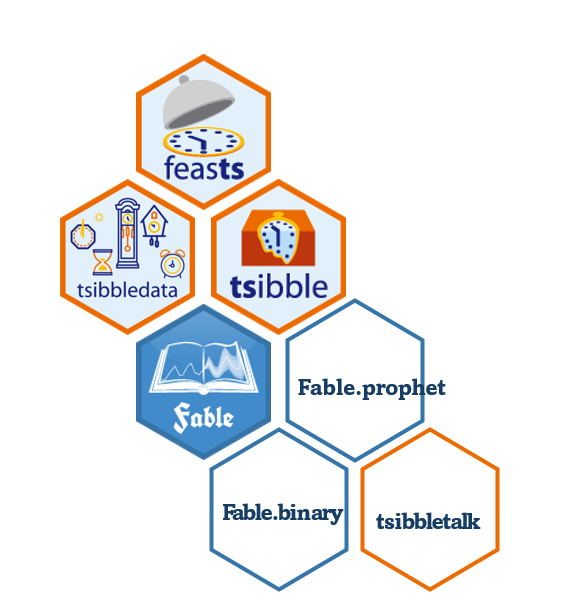
\includegraphics[keepaspectratio]{images/clipboard-351646644.png}}

}

\caption{Tidyverts Package Collection}

\end{figure}%%
\begin{figure}[H]

{\centering \pandocbounded{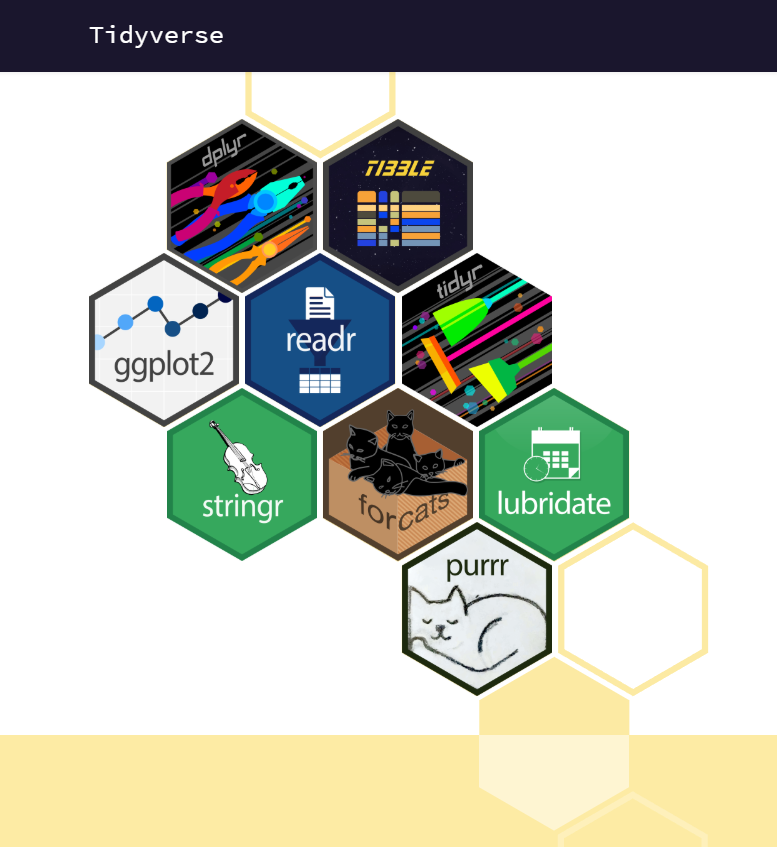
\includegraphics[keepaspectratio]{images/clipboard-419927233.png}}

}

\caption{Tidyverse Package Collection}

\end{figure}%

This section will cover installing and loading the packages we will use
and checking that your R environment is prepared for a smooth time
series work

We will address the following:

\begin{itemize}
\tightlist
\item
  Chapter~\ref{sec-required-packages}: This part will cover all the
  packages we will need, how to install and load them for use in our R
  environment.
\item
  Chapter~\ref{sec-setting-up-your-rstudio-environment}: Here you will
  see how to keep things organised in a more seamless and orderly manner
  on your system.
\end{itemize}

After going through this section you should have been able to
\textbf{install and load} all required packages, make RStudio
r\textbf{eady for your time series coding} and then been able able to
\textbf{successfully load a test} dataset.

\chapter{Required Packages}\label{sec-required-packages}

As stated earlier we will be using a combination of \texttt{tidyverse}
and time series specific packages (\texttt{tidyverts})

\begin{longtable}[]{@{}
  >{\raggedright\arraybackslash}p{(\linewidth - 2\tabcolsep) * \real{0.2083}}
  >{\raggedright\arraybackslash}p{(\linewidth - 2\tabcolsep) * \real{0.7917}}@{}}
\toprule\noalign{}
\begin{minipage}[b]{\linewidth}\raggedright
Package
\end{minipage} & \begin{minipage}[b]{\linewidth}\raggedright
Purpose
\end{minipage} \\
\midrule\noalign{}
\endhead
\bottomrule\noalign{}
\endlastfoot
\texttt{tidyverse} & Core suite for data wrangling and visualisation
(\texttt{dplyr}, \texttt{tibble}, \texttt{ggplot2}, \texttt{readr},
etc) \\
\texttt{tsibble} & Tidy data frames for time series, handles dates, keys
and indexing \\
\texttt{fable} & Forecasting models (ETS, ARIMA, Naive, etc) with tidy
outputs \\
\texttt{feasts} & \textbf{F}eature \textbf{E}xtraction and
\textbf{A}nalysis for \textbf{S}eries \textbf{T}ime \textbf{S}eries
(plots, decomposition, autocorrelation, etc) \\
\texttt{lubridate} & Easy and readable date time manipulation \\
\texttt{readr} & Fast and easy data imports (csv, text data, etc) \\
\texttt{readxl} & Importing excel files (could be optional but very
useful) \\
\end{longtable}

\begin{tcolorbox}[enhanced jigsaw, rightrule=.15mm, opacitybacktitle=0.6, breakable, colframe=quarto-callout-note-color-frame, opacityback=0, colbacktitle=quarto-callout-note-color!10!white, leftrule=.75mm, titlerule=0mm, toprule=.15mm, coltitle=black, colback=white, bottomrule=.15mm, left=2mm, bottomtitle=1mm, arc=.35mm, toptitle=1mm, title=\textcolor{quarto-callout-note-color}{\faInfo}\hspace{0.5em}{Note}]

the \texttt{readr} and \texttt{lubridate} packages are already part of
the \textbf{tidyverse package collections}. Once you install
\texttt{tidyverse}, you do not need to install them again separately.

\end{tcolorbox}

\section{Installing the Package}\label{installing-the-package}

\chapter{Setting Up Your RStudio
Environment}\label{sec-setting-up-your-rstudio-environment}

\part{Working with Time Series in \texttt{tsibble}}

\chapter{Tidy Time Series Basics}\label{tidy-time-series-basics}

\chapter{Dealing with Time Gaps and
Irregularities}\label{dealing-with-time-gaps-and-irregularities}

\chapter{Importing Data and Creating a
tsibble}\label{importing-data-and-creating-a-tsibble}

\bookmarksetup{startatroot}

\chapter*{References}\label{references}
\addcontentsline{toc}{chapter}{References}

\markboth{References}{References}

\phantomsection\label{refs}
\begin{CSLReferences}{0}{1}
\end{CSLReferences}




\end{document}
